%!TEX root = main.tex
\begin{figure*}[htb]
    \centering
    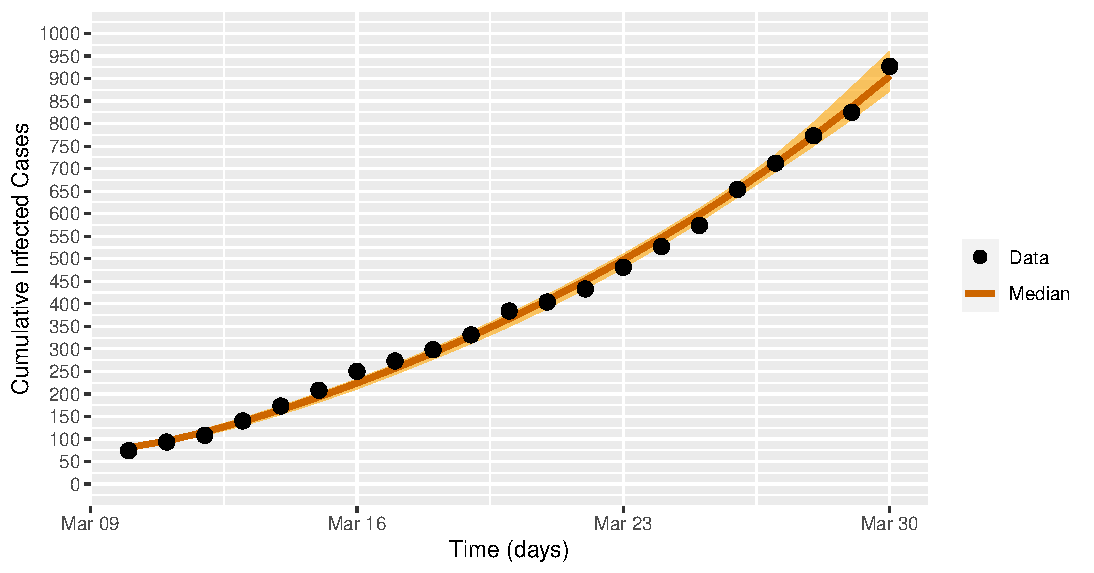
\includegraphics[scale=0.7, keepaspectratio]{./cdmx_CIs_data_begining_fit}
    \caption{%
        Fit of daily new cases of Mexico city
        during exponential growth.
        \href{https://plotly.com/~AdrianSalcedo/50/}{%
		 https://plotly.com/~AdrianSalcedo/50/}
    }
    \label{fig:data_CDMX_fitting}
\end{figure*}
%

\paragraph{Bayesian estimation}

We calibrate parameters of our base dynamics
\eqref{eqn:base_dynamics} via Multichain Montecarlo (MCMC).
To this end, we assume that the cumulative
incidence of new infected symptomatic cases $CI_S$
follows a Poisson distribution with mean $\lambda_t = IC_s(t)$. Further,
following [] we postulate priors for $p$ and $\kappa$
\begin{equation}
    \label{eqn:boservation_model}
    \begin{aligned}
        Y_t & \sim Poisson(\lambda_t),
        \\
        \lambda_t
        &=
        \int_{0}^t p \delta_e E ,
        \\
        & p \sim \text{Uniform} (0.3, 0.8),
        \\
        & \kappa \sim \text{Gamma}(10, 50).
    \end{aligned}
\end{equation}
%
\comment[id=SDIV]{Review this $R_0$ calculation with Gabriel}

\Cref{fig:data_CDMX} displays data of cumulative confirmed cases
of COVID-19 in Mexico city, and \Cref{fig:data_CDMX_fitting} displays the fitted curve
of our model in \Cref{eqn:base_dynamics,eqn:boservation_model}.
\Cref{tbl:parameters_values} encloses estimated parameters to this
setting.

  \begin{table*}
    \centering
    \begin{tabular}{@{}llr@{}}
    \toprule
        Parameter
        &   \centering{Median}
        &   Reference
        \\
        \midrule
          $q_r$, $\epsilon$
            &
              \num{.4}, \num{.3}, \num{.1}
            &
              this study
        \\
            $\beta_S$
            & $q_r \times \num{8.690483e-01} $
            & this study
        \\
            $\beta_A$
            & $q_r \times \num{7.738431e-01}$
            & this study

        \\
            $\kappa$
            & \num{0.19607843}
            & $*$
        \\
            $p$
            & \num{0.1213}
            & $*$
        \\
          $\theta$
          & \num{0.2},
          & this study
        \\
          $\delta_L$
          & \num{0.04}
          & postulated
        \\
            $\delta_H$
            &\num{0.2}
            & $*$
        \\
          $\delta_V$
          &\num{ 0.0027397260273972603}
          & $\delta_V ^{-1} = \SI{2}{years}$
        \\
        &&
            CanSinoBIO
        \\
          $\delta_R$
          & \num{0.00555556}
          & $\delta_R^{-1} \approx \SI{180}{days}$
        \\
            $\mu$
            & \num{ 3.913894e-05}
            & $**$
        \\
            $\mu_{I_S}$
            & \num{0.0}
            &
        \\
            $\mu_{H}$
            & \num{0.01632}
            & \cite{Zhao2020}
        \\
            $\gamma_S$
            & \num{0.09250694}
            & $*$
        \\
             $\gamma_A$
             & \num{0.16750419}
             & $*$
        \\
           $\gamma_H$
            & \num{5.079869e-01}
            & $*$
        \\
          $\lambda_V$
          &  \num{0.00061135}
          &
        \\
          $\varepsilon$
          & \num{0.7}, \num{0.80}, \num{0.9}, \num{0.95}
          & [PRESS RELESASES]
        \\
        \midrule
            $N$
             & \num{26446435}
             & $**$
        \\
            $L_0$
            & \num{0.26626009702112796}
        \\
            $S_0$
             & \num{0.463606046009872}
             &
        \\
            $E_0$
             & \num{0.00067033}
             & $*$
        \\
            $I_{S_0}$
            & \num{9.283e-05}
            & $***$
        \\
            $I_{A_0}$
            & \num{0.00120986}
            & $*$
        \\
            $H_0$
            & \num{1.34157969e-04}
            & $**$
        \\
            $R_0$
            & \num{2.66125939e-01}
            &
        \\
            $D_0$
            & \num{0.00190074}
            & $**$
        \\
            $X_{vac}^0$
            & 0.0
        \\
            $V_0$
            & 0.0
        \\
            $Y_{I_S} ^ 0$ &
            \num{0.12258164}
        \\
            $B$
        &
            \num{0.0003592166581242425}
        &
            $
                \displaystyle
                \SI{9500}{beds} / {N}
            $
        \\
          $a_{I_S}$
            & \num{0.0020127755438256486}
            & DALY def
        \\
          $a_{H}$
            & \num{0.001411888738103725},
            or
        \\
        & $
            a_H(x):=
            \num{0.001411888738103725}
            \log(\frac{1}{B - \kappa I_S})
        $
        & DALY def [Jo 2020]
        \\
            $a_D$
            & \num{7.25}
            & DALY def
      \\
        \bottomrule
    \end{tabular}
    \caption{Model parameters. Values based mainly in [FNEG]}
    \label{tbl:parameters_values}
\end{table*}